%
% ---------------------------------------------------------------
% Copyright (C) 2012-2018 Gang Li
% ---------------------------------------------------------------
%
% This work is the default powerdot-tuliplab style test file and may be
% distributed and/or modified under the conditions of the LaTeX Project Public
% License, either version 1.3 of this license or (at your option) any later
% version. The latest version of this license is in
% http://www.latex-project.org/lppl.txt and version 1.3 or later is part of all
% distributions of LaTeX version 2003/12/01 or later.
%
% This work has the LPPL maintenance status "maintained".
%
% This Current Maintainer of this work is Gang Li.
%
%

\documentclass[
 size=12pt,
 paper=smartboard,  %a4paper, smartboard, screen
 mode=present, 		%present, handout, print
 display=slides, 	% slidesnotes, notes, slides
 style=tuliplab,  	% TULIP Lab style
 pauseslide,
 fleqn,leqno]{powerdot}


\usepackage{cancel}
\usepackage{caption}
\usepackage{stackengine}
\usepackage{smartdiagram}
\usepackage{attrib}
\usepackage{amssymb}
\usepackage{amsmath} 
\usepackage{amsthm} 
\usepackage{mathtools}
\usepackage{rotating}
\usepackage{graphicx}
\usepackage{boxedminipage}
\usepackage{rotate}
\usepackage{calc}
\usepackage[absolute]{textpos}
\usepackage{psfrag,overpic}
\usepackage{fouriernc}
\usepackage{pstricks,pst-3d,pst-grad,pstricks-add,pst-text,pst-node,pst-tree}
\usepackage{moreverb,epsfig,subfigure}
\usepackage{color}
\usepackage{booktabs}
\usepackage{etex}
\usepackage{breqn}
\usepackage{multirow}
\usepackage{natbib}
\usepackage{bibentry}
\usepackage{gitinfo2}
\usepackage{siunitx}
\usepackage{nicefrac}
%\usepackage{geometry}
%\geometry{verbose,letterpaper}
\usepackage{media9}
\usepackage{animate}
%\usepackage{movie15}
\usepackage{auto-pst-pdf}

\usepackage{breakurl}
\usepackage{fontawesome}
\usepackage{xcolor}
\usepackage{multicol}



\usepackage{verbatim}
\usepackage[utf8]{inputenc}
\usepackage{dtk-logos}
\usepackage{tikz}
\usepackage{adigraph}
%\usepackage{tkz-graph}
\usepackage{hyperref}
%\usepackage{ulem}
\usepackage{pgfplots}
\usepackage{verbatim}
\usepackage{fontawesome}


\usepackage{todonotes}
% \usepackage{pst-rel-points}
\usepackage{animate}
\usepackage{fontawesome}

\usepackage{listings}
\lstset{frameround=fttt,
frame=trBL,
stringstyle=\ttfamily,
backgroundcolor=\color{yellow!20},
basicstyle=\footnotesize\ttfamily}
\lstnewenvironment{code}{
\lstset{frame=single,escapeinside=`',
backgroundcolor=\color{yellow!20},
basicstyle=\footnotesize\ttfamily}
}{}


\usepackage{hyperref}
\hypersetup{ % TODO: PDF meta Data
  pdftitle={Recent Work},
  pdfauthor={Huanhuan Ge},
  pdfpagemode={FullScreen},
  pdfborder={0 0 0}
}
\usepackage{setspace} 

% \usepackage{auto-pst-pdf}
% package to show source code

\definecolor{LightGray}{rgb}{0.9,0.9,0.9}
\newlength{\pixel}\setlength\pixel{0.000714285714\slidewidth}
\setlength{\TPHorizModule}{\slidewidth}
\setlength{\TPVertModule}{\slideheight}
\newcommand\highlight[1]{\fbox{#1}}
\newcommand\icite[1]{{\footnotesize [#1]}}

\newcommand\twotonebox[2]{\fcolorbox{pdcolor2}{pdcolor2}
{#1\vphantom{#2}}\fcolorbox{pdcolor2}{white}{#2\vphantom{#1}}}
\newcommand\twotoneboxo[2]{\fcolorbox{pdcolor2}{pdcolor2}
{#1}\fcolorbox{pdcolor2}{white}{#2}}
\newcommand\vpspace[1]{\vphantom{\vspace{#1}}}
\newcommand\hpspace[1]{\hphantom{\hspace{#1}}}
\newcommand\COMMENT[1]{}

\newcommand\placepos[3]{\hbox to\z@{\kern#1
        \raisebox{-#2}[\z@][\z@]{#3}\hss}\ignorespaces}

% \renewcommand{\baselinestretch}{1.2}
\renewcommand{\baselinestretch}{1.2}

\newcommand{\draftnote}[3]{
	\todo[author=#2,color=#1!30,size=\footnotesize]{\textsf{#3}}	}
% TODO: add yourself here:
%
\newcommand{\gangli}[1]{\draftnote{blue}{GLi:}{#1}}
\newcommand{\shaoni}[1]{\draftnote{green}{sn:}{#1}}
\newcommand{\gliMarker}
	{\todo[author=GLi,size=\tiny,inline,color=blue!40]
	{Gang Li has worked up to here.}}
\newcommand{\snMarker}
	{\todo[author=Sn,size=\tiny,inline,color=green!40]
	{Shaoni has worked up to here.}}

%%%%%%%%%%%%%%%%%%%%%%%%%%%%%%%%%%%%%%%%%%%%%%%%%%%%%%%%%%%%%%%%%%%%%%%%
% title
% TODO: Customize to your Own Title, Name, Address
%
\title{FLIP00 Midterm Presentation}
\author{
Huanhuan Ge
\\
\\Qingdao University of Technology
}
\date{\gitCommitterDate}


% Customize the setting of slides
\pdsetup{
% TODO: Customize the left footer, and right footer
rf=\href{http://www.tulip.org.au}{
Last Changed by: \textsc{\gitCommitterDate}
},
cf={FLIP00 Midterm Presentation},
}


\begin{document}

\maketitle


%%==========================================================================================
%%
\begin{slide}[toc=,bm=]{Overview}
\begin{spacing}{1.00}
\tableofcontents[content=currentsection,type=1]
\end{spacing}
\end{slide}
%%
%%==========================================================================================


\section{Recent Work}


%%==========================================================================================
%%
\begin{slide}{Latex}
\begin{center}
\begin{itemize}
  \item
  Building the latex compilation environment
  \item
  Basic grammar and usage
  \begin{itemize}
    \item
    Fonts, Chapters, Math Formulas
    \item
    Table,Picture
  \end{itemize}
  \item
  Use of Report, Poster, Slide templates  
\end{itemize}
\end{center}
%%==========================================================================================
\begin{note}
First, I will introduce the problem definition.
\end{note}
%%==========================================================================================

\end{slide}
%%
%%==========================================================================================


%%==========================================================================================
%%
% \section{Git}

\begin{slide}{Git}
  \begin{itemize}
    \item
    Common commands of Git. 
    \begin{itemize}
      \item
      git add,git commit,git push
    \end{itemize}
    \item 
    git-flow,git latexdiff
  \end{itemize}
  \vspace{0.75cm}
      
    \twocolumn{
      \begin{figure}
        \centering
        % \selectcolormodel{rgb}
        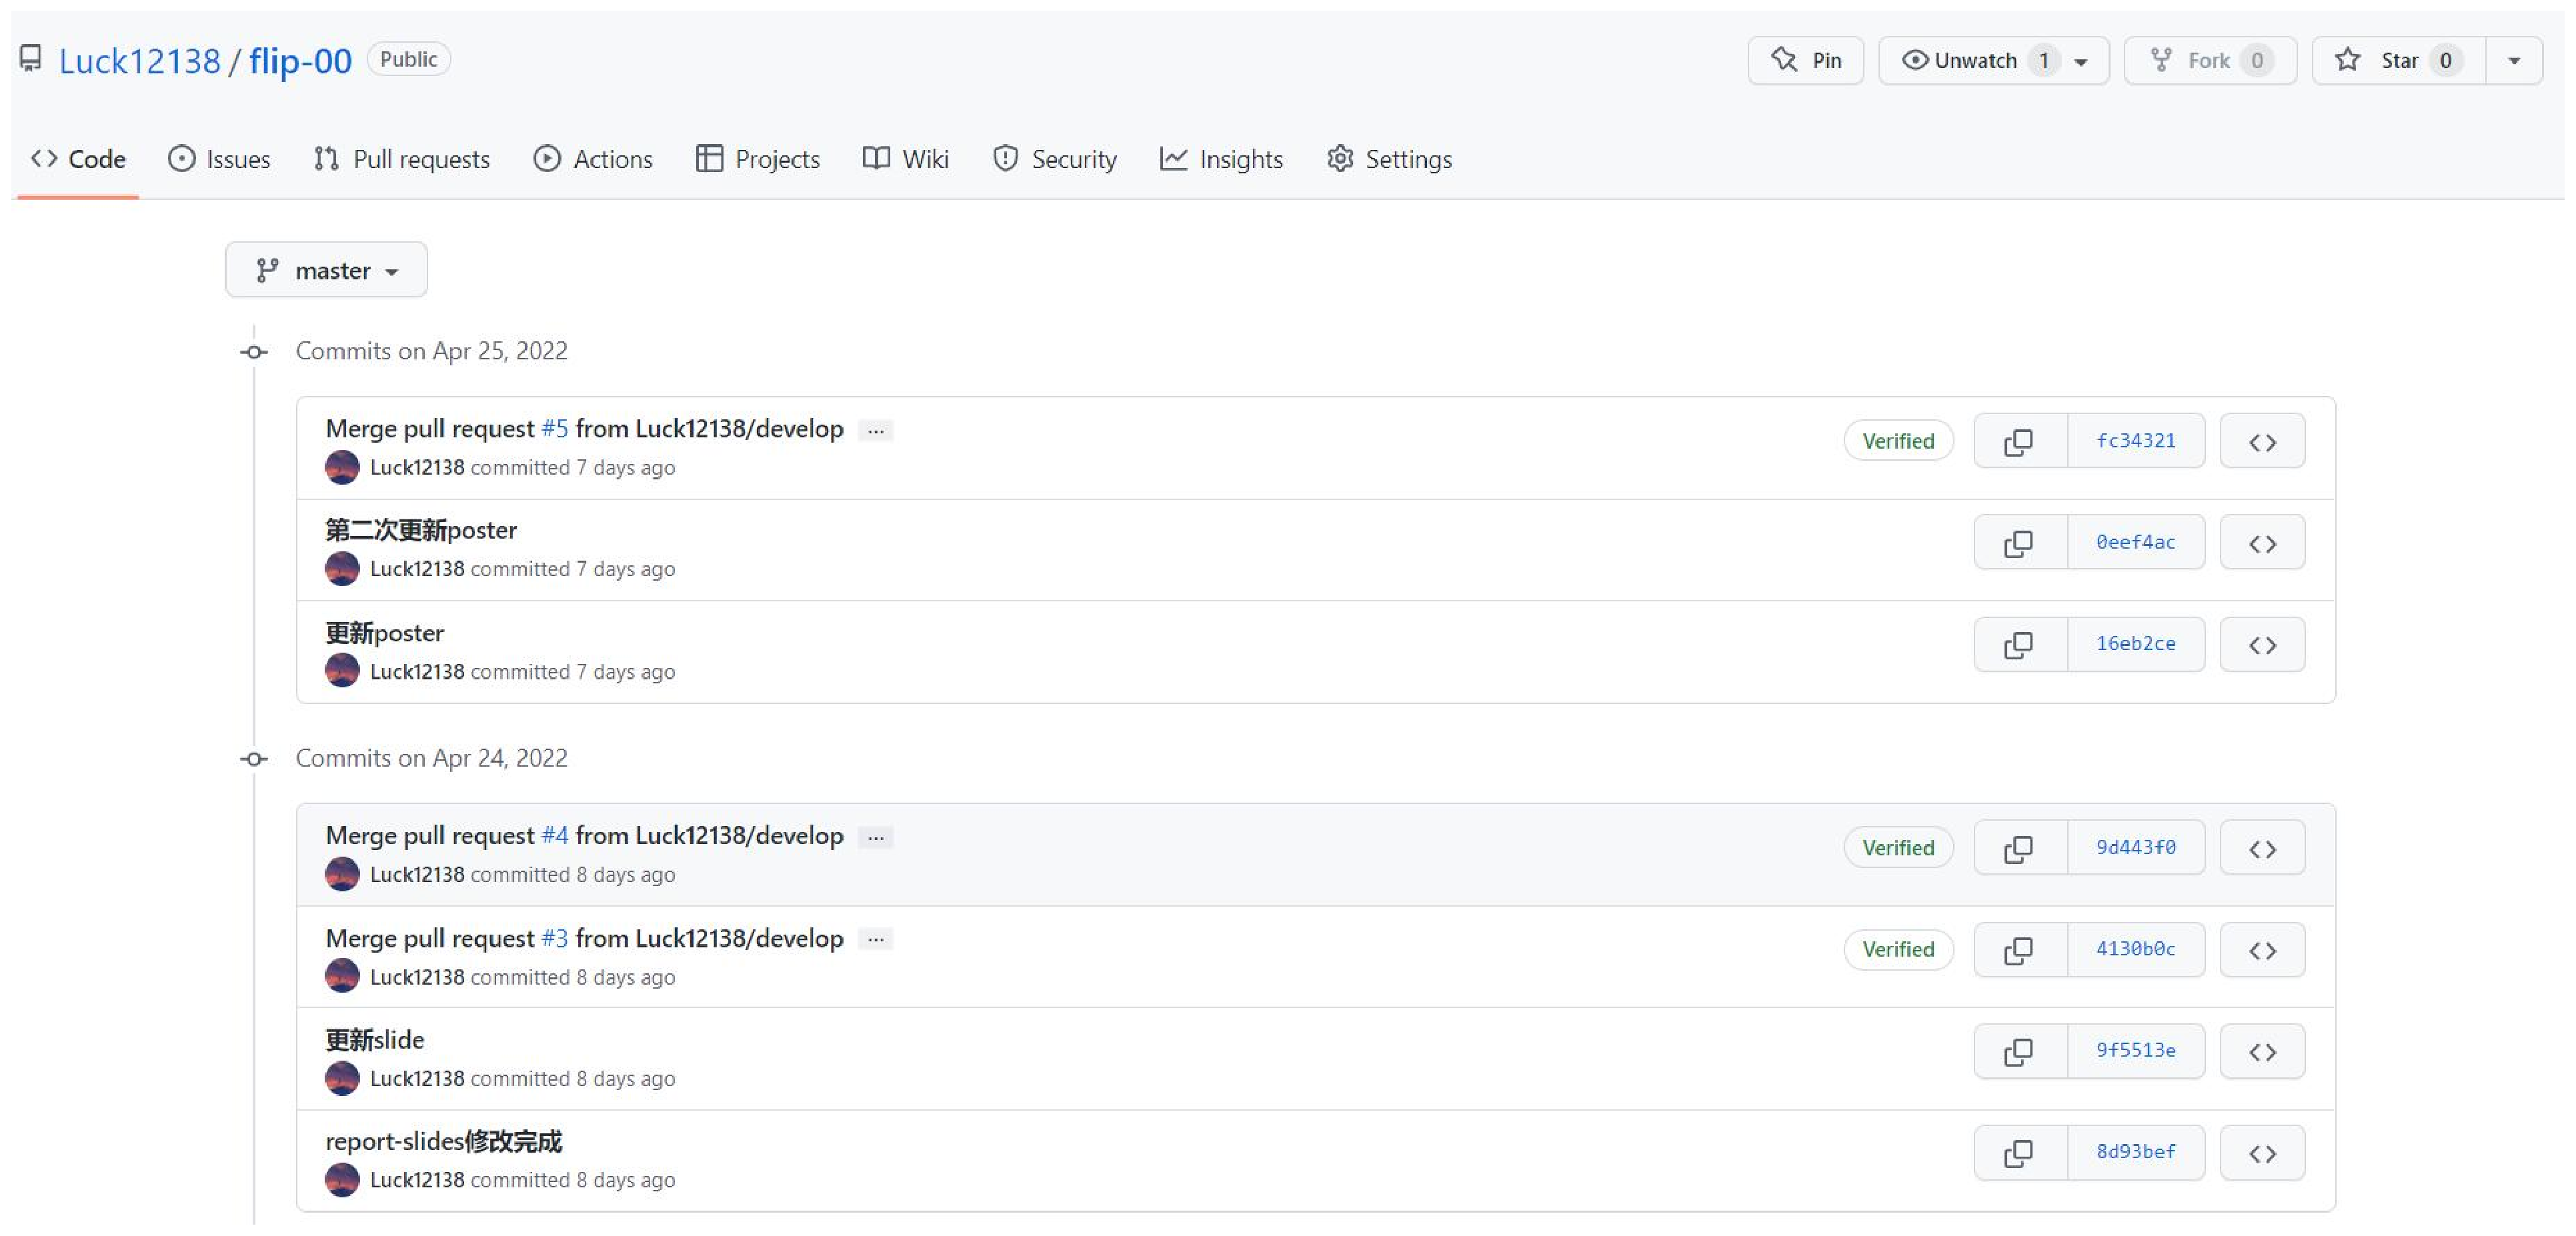
\includegraphics[width=1.0\textwidth,height=0.8\textwidth]{figures/first-meeting1.eps}\\
        \caption{Pull Request Recode}
      \end{figure}
      }{
      \begin{figure}
        \centering
        % \selectcolormodel{rgb}
        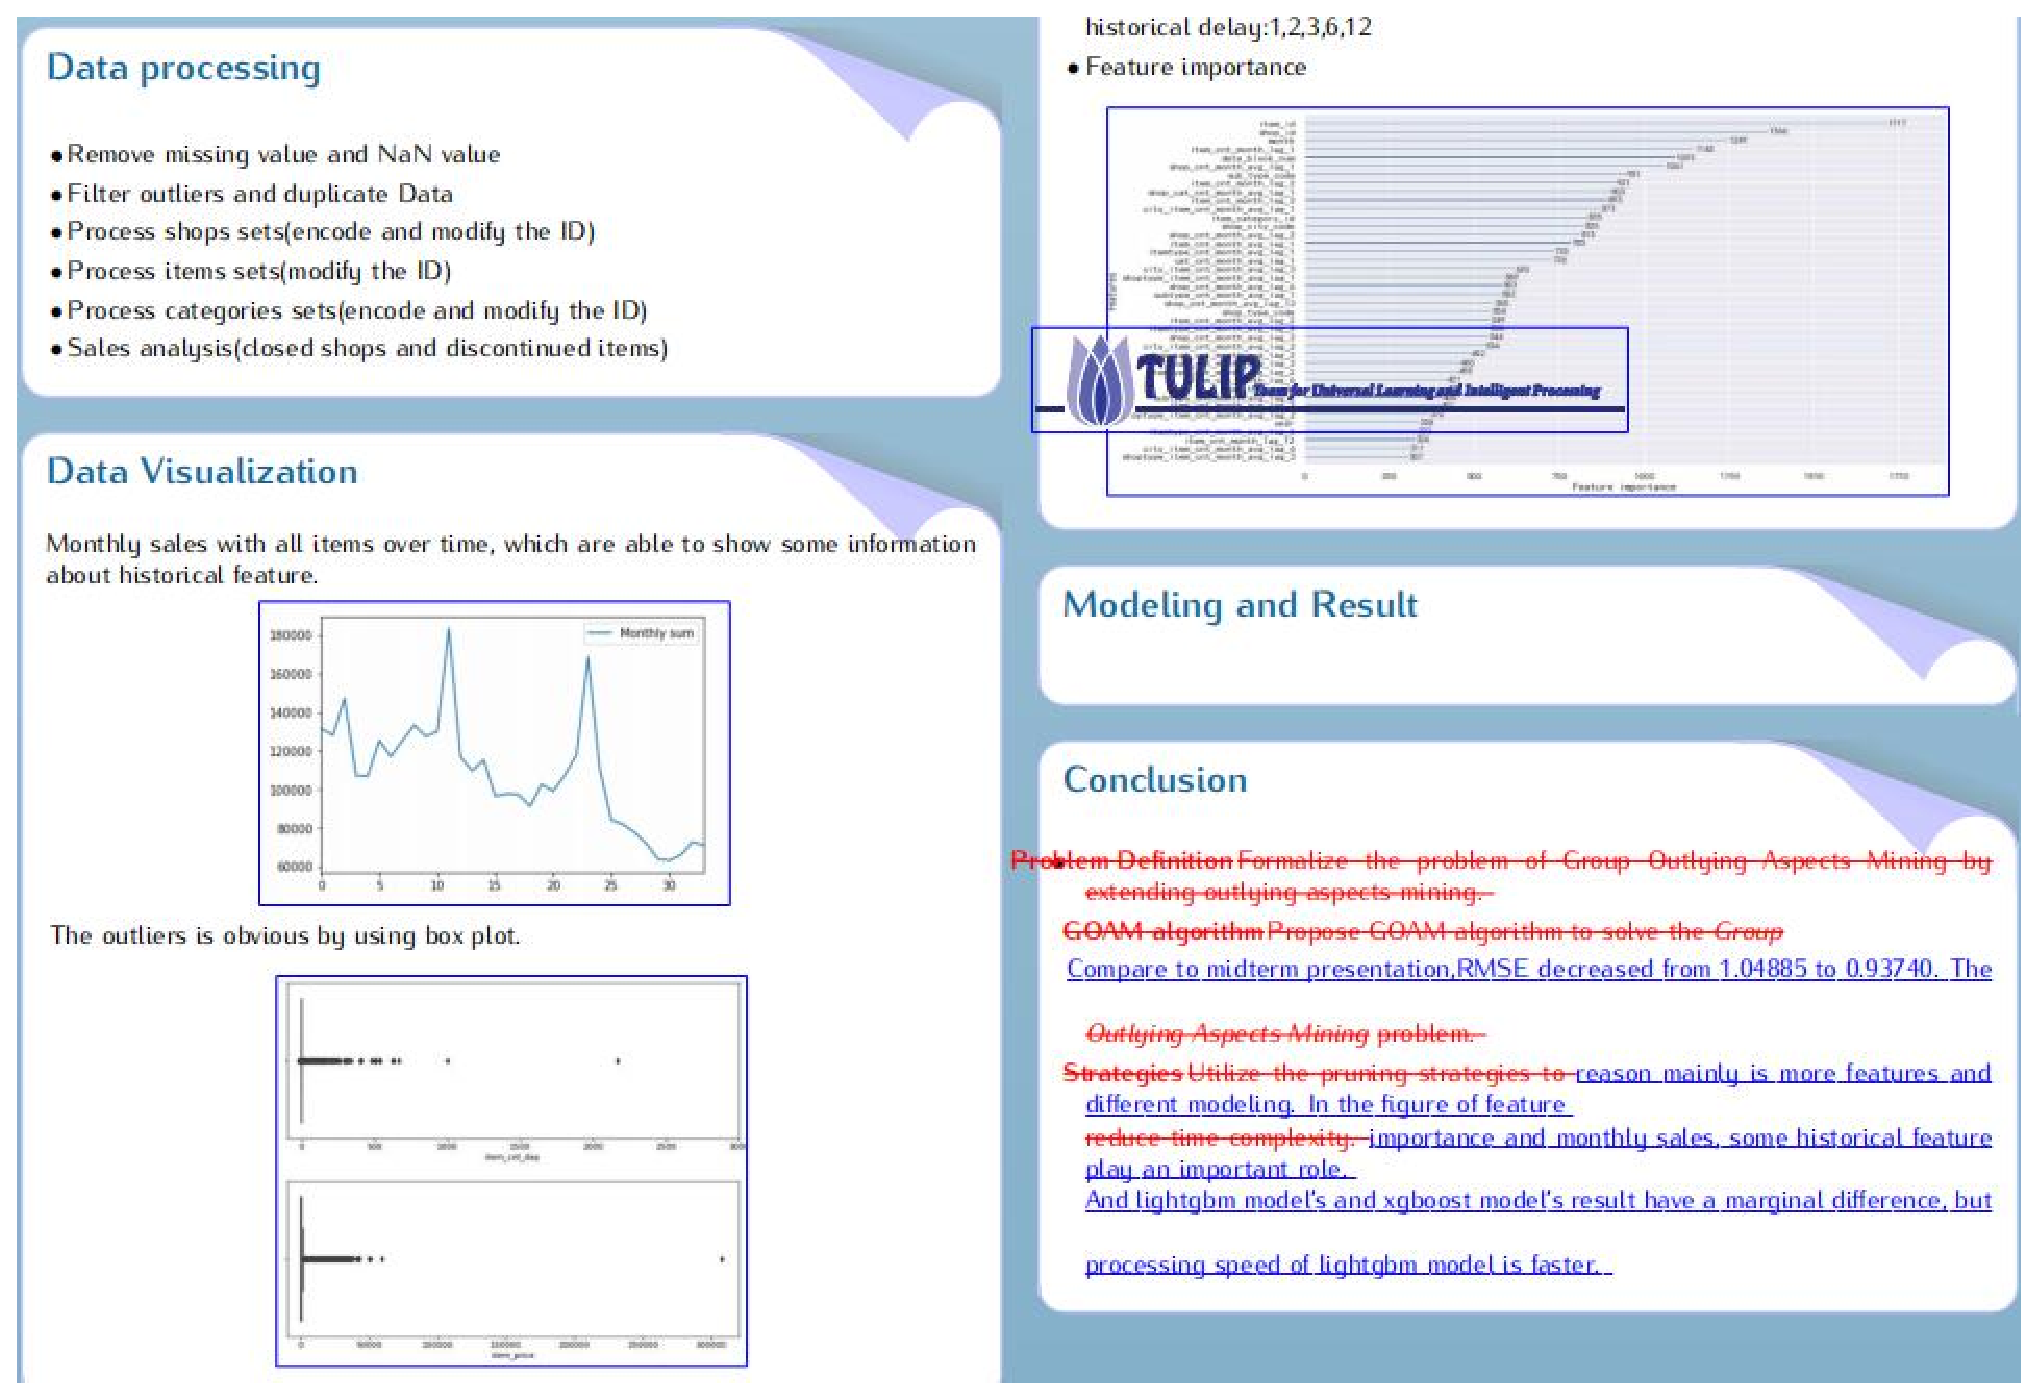
\includegraphics[width=1.0\textwidth,height=0.8\textwidth]{figures/first-meeting2.eps}\\
        \caption{latexdiff example}
      \end{figure}
      }



%%==========================================================================================
\begin{note}
Based on the above example,
\end{note}
%%==========================================================================================

\end{slide}
%%
%%==========================================================================================

%%

%%==========================================================================================
%%
\begin{slide}{Data Science}
  \begin{center}
  \begin{itemize}
    \item
    Data processing method and flow
    \item
    Machine Learing
    \begin{itemize}
      \item
      KNN,LinearRegression
      \item
      Kmeans,PCA
    \end{itemize}
    \bigskip
    \item
    python environment construction and basic syntax
    \item
    Math,Numpy,Pandas,Matplotlib...
    \item
    python data visualization
    \begin{itemize}
      \item
    %  饼图
      Pie Chart, Bar Chart,Step Plot,Histogram,Scatter Plot
    \end{itemize}
  \end{itemize}
  \end{center}
  %%==========================================================================================
  \begin{note}
  First, I will introduce the problem definition.
  \end{note}
  %%==========================================================================================
  
  \end{slide}

%%==========================================================================================
%%
\section{The next work}

\begin{slide}{The next work}
  \begin{center}
  \begin{itemize}
    \item
    PDM,Python NoteBook
    \item
    Linear Algebra
    \item
     Prabability Theory
  \end{itemize}
  \end{center}
  %%==========================================================================================
  \begin{note}
  First, I will introduce the problem definition.
  \end{note}
  %%==========================================================================================

  \end{slide}

%%
%%==========================================================================================


%%
%%==========================================================================================

%%
% TODO: Contact Page
% \begin{wideslide}[toc=,bm=]{Contact Information}
% \centering
% \vspace{\stretch{1}}
% \twocolumn[
% lcolwidth=0.35\linewidth,
% rcolwidth=0.65\linewidth
% ]
% {
% % \centerline{
\includegraphics[scale=.2]{tulip-logo.eps}}
% }
% {
% \vspace{\stretch{1}}
% Associate Professor Gang Li\\
% School of Information Technology\\
% Deakin University, Australia
% \begin{description}
%  \item[\textcolor{orange}{\faEnvelope}] \href{mailto:gangli@tulip.org.au}
%  {\textsc{\footnotesize{gangli@tulip.org.au}}}

%  \item[\textcolor{orange}{\faHome}] \href{http://www.tulip.org.au}
%  {\textsc{\footnotesize{Team for Universal Learning and Intelligent Processing}}}
% \end{description}
% }
% \vspace{\stretch{1}}
% \end{wideslide}

\end{document}

\endinput
